% Copyright 2006 by Till Tantau
%
% This file may be distributed and/or modified
%
% 1. under the LaTeX Project Public License and/or
% 2. under the GNU Free Documentation License.
%
% See the file doc/generic/pgf/licenses/LICENSE for more details.

\section{Making Trees Grow}

\label{section-trees}


\subsection{Introduction to the  Child Operation}

\emph{Trees} are a common way of visualizing hierarchical
structures. A simple tree looks like this:
\begin{codeexample}[]
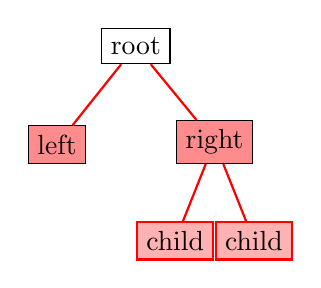
\begin{tikzpicture}
  \node {root}
    child {node {left}}
    child {node {right}
      child {node {child}}
      child {node {child}}
    };
\end{tikzpicture}
\end{codeexample}

Admittedly, in reality trees are more likely to grow \emph{upward} and
not downward as above. You can tell whether the author of a paper is a
mathematician or a computer scientist by looking at the direction
their trees grow. A computer scientist's trees will grow downward
while a mathematician's tree will grow upward. Naturally, the
\emph{correct} way is the mathematician's way, which can be specify as
follows: 
\begin{codeexample}[]
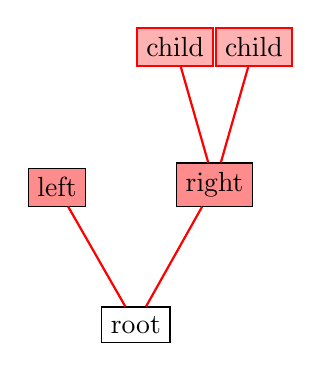
\begin{tikzpicture}
  \node {root} [grow'=up]
    child {node {left}}
    child {node {right}
      child {node {child}}
      child {node {child}}
    };
\end{tikzpicture}
\end{codeexample}

In \tikzname, trees are specified by adding \emph{children} to a
node on a path using the |child| operation:

\begin{pathoperation}{child}{\opt{\oarg{options}}%
    \opt{|foreach|\meta{variables}|in|\marg{values}}\opt{\marg{child path}}} 
  This operation should directly follow a completed |node| operation
  or another |child| operation, although it is permissible that the
  first |child| operation is preceded by options (we will come to
  that).

  When a |node| operation like |node {X}| is followed by |child|,
  \tikzname\ starts counting the number of child nodes that follow the
  original |node {X}|. For this, it scans the input and stores away each
  |child| and its arguments until it reaches a path operation that is
  not a |child|. Note that this will fix the character codes of all
  text inside the child arguments, which means, in essence, that you
  cannot use verbatim text inside the nodes inside a |child|. Sorry. 

  Once the children have been collected and counted, \tikzname\ starts
  generating the child nodes. For each child of a parent node
  \tikzname\ computes an appropriate position where the child is
  placed. For each child, the coordinate system is transformed so that
  the origin is at this position. Then the \meta{child path} is
  drawn. Typically, the child path just consists of a |node|
  specification, which results in a node being drawn at the child's
  position. Finally, an edge is drawn from the first node in the
  \meta{child path} to the parent node.

  The optional |foreach| part (note that there is no backslash before
  |foreach|) allows you to specify multiple children in a single
  |child| command. The idea is the following: A |\foreach| statement
  is (internally) used to iterate over the list of \meta{values}. For
  each value in this list, a new |child| is added to the node. The
  syntax for \meta{variables} and for \meta{values} is the same as for
  the |\foreach| statement, see Section~\ref{section-foreach}. For
  example, when you say 
\begin{codeexample}[code only]
node {root} child [red] foreach \name in {1,2} {node {\name}}
\end{codeexample}
  the effect will be the same as if you had said
\begin{codeexample}[code only]
node {root} child[red] {node {1}} child[ref] {node {2}}
\end{codeexample}
  When you write 
\begin{codeexample}[code only]
node {root} child[\pos] foreach \name/\pos in {1/left,2/right} {node[\pos] {\name}}
\end{codeexample}
  the effect will be the same as for
\begin{codeexample}[code only]
node {root} child[left] {node[left] {1}} child[right] {node[right] {2}}
\end{codeexample}

  You can nest things as in the following example:
\begin{codeexample}[]
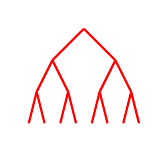
\begin{tikzpicture}[level distance=4mm]
  \tikzstyle{level 1}=[sibling distance=8mm]
  \tikzstyle{level 2}=[sibling distance=4mm]
  \tikzstyle{level 3}=[sibling distance=2mm]
  \coordinate
    child foreach \x in {0,1}
      {child foreach \y in {0,1} 
        {child foreach \z in {0,1}}};
\end{tikzpicture}
\end{codeexample}

  The details and options for this operation are described in the rest
  of this present section.
\end{pathoperation}



\subsection{Child Paths and the Child Nodes}

For each |child| of a root node, its \meta{child path} is inserted at
a specific location in the picture (the placement rules are discussed
in Section~\ref{section-tree-placement}). The first node in the
\meta{child path}, if it exists, is special and called the \emph{child
  node}. If there is no first node in the \meta{child path}, that is,
if the \meta{child path} is missing (including the curly braces) or if
it does not start with |node| or with |coordinate|, then an empty
child node of shape |coordinate| is automatically added.

Consider the example |\node {x} child {node {y}} child;|. For the
first child, the \meta{child path} has the child node |node {y}|. For
the second child, no child node is specified and, thus, it is just
|coordinate|.

As for any normal node, you can give the child node a name, shift it 
around, or use options to influence how it is rendered.
\begin{codeexample}[]
\begin{tikzpicture}
  \node[rectangle,draw] {root}
    child {node[circle,draw] (left node) {left}}
    child {node[ellipse,draw] (right node) {right}};
  \draw[dashed,->] (left node) -- (right node);
\end{tikzpicture}
\end{codeexample}

In many cases, the \meta{child path} will just consist of a
specification of a child node and, possibly, children of this child
node. However, the node specification may be followed by arbitrary
other material that will be added to the picture, transformed to the
child's coordinate system. For your convenience, a move-to |(0,0)|
operation is inserted automatically at the beginning of the path. Here
is an example: 

\begin{codeexample}[]
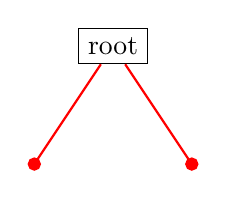
\begin{tikzpicture}
  \node {root}
    child {[fill] circle (2pt)}
    child {[fill] circle (2pt)};
\end{tikzpicture}    
\end{codeexample}


At the end of the \meta{child path} you may add a special path
operation called |edge from parent|. If this operation is not given by
yourself somewhere on the path, it will be automatically added at the
end. This option causes a connecting edge from the parent node to the
child node to be added to the path. By giving options to this
operation you can influence how the edge is rendered. Also, nodes
following the |edge from parent| operation will be placed on this
edge, see Section~\ref{section-edge-from-parent} for details.

To sum up:
\begin{enumerate}
\item
  The child path starts with a node specification. If it is not there,
  it is added automatically.
\item
  The child path ends with a |edge from parent| operation, possibly
  followed by nodes to be put on this edge. If the operation is not
  given at the end, it is added automatically.
\end{enumerate}



\subsection{Naming Child Nodes}

Child nodes can be named like any other node using either the |name|
option or the special syntax in which the name of the node is placed
in round parentheses between the |node| operation and the node's
text.

If you do not assign a name to a child node, \tikzname\ will
automatically assign a name as follows: Assume that the name of the
parent node is, say, |parent|. (If you did not assign a
name to the parent, \tikzname\ will do so itself, but that name will
not be user-accessible.) The first child
of |parent| will be named |parent-1|, the second child is named
|parent-2|, and so on.

This naming convention works recursively. If the second child
|parent-2| has children, then the first of these children will be
called |parent-2-1| and the second |parent-2-2| and so on.

If you assign a name to a child node yourself, no name is generated
automatically (the node does not have two names). However, ``counting
continues,'' which means that the third child of |parent| is called
|parent-3| independently of whether you have assigned names to the
first and/or second child of |parent|.

Here is an example:

\begin{codeexample}[]
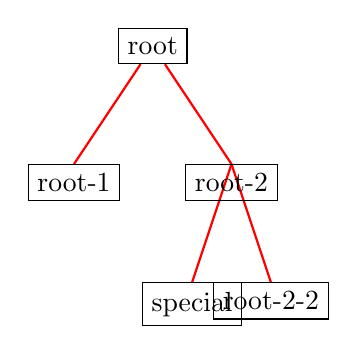
\begin{tikzpicture}
  \node (root) {root}
    child 
    child {
      child {coordinate (special)}
      child
    };
  \node at (root-1) {root-1};
  \node at (root-2) {root-2};
  \node at (special) {special};
  \node at (root-2-2) {root-2-2};
\end{tikzpicture}
\end{codeexample}

\subsection{Specifying Options for Trees and Children}

Each |child| may have its own \meta{options}, which apply to ``the
whole child,'' including all of its grandchildren. Here is an
example:

\begin{codeexample}[]
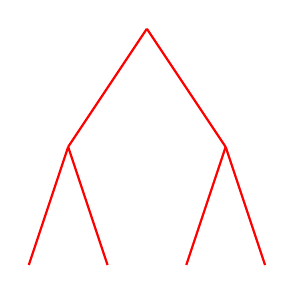
\begin{tikzpicture}[thick]
  \tikzstyle{level 2}=[sibling distance=10mm]
  \coordinate
    child[red]   {child child}
    child[green] {child child[blue]};
\end{tikzpicture}
\end{codeexample}

The options of the root node have no effect on the children since
the options of a node are always ``local'' to that node. Because of
this, the edges in the following tree are black, not red.
  
\begin{codeexample}[]
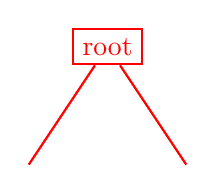
\begin{tikzpicture}[thick]
  \node [red] {root}
    child
    child;
\end{tikzpicture}
\end{codeexample}
  This raises the problem of how to set options for \emph{all}
  children. Naturally, you could always set options for the whole path
  as in |\path [red] node {root} child child;| but this is bothersome
  in some situations. Instead, it is easier to give the options
  \emph{before the first child} as follows:
\begin{codeexample}[]
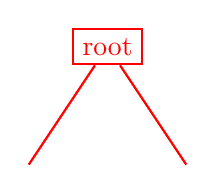
\begin{tikzpicture}[thick]
  \node [red] {root}
    [green] % option applies to all children
    child
    child;
\end{tikzpicture}
\end{codeexample}

Here is the set of rules:
\begin{enumerate}
\item
  Options for the whole tree are given before the root node.
\item
  Options for the root node are given directly to the |node| operation
  of the root.
\item
  Options for all children can be given between the root node and the
  first child.
\item
  Options applying to a specific child path are given as options to
  the |child| operation.
\item
  Options applying to the node of a child, but not to the whole child
  path, are given as options to the |node| command inside the
  \meta{child path}.
\end{enumerate}

\begin{codeexample}[code only]
\begin{tikzpicture}
  \path
    [...]             % Options apply to the whole tree
    node[...] {root}  % Options apply to the root node only
      [...]           % Options apply to all children
      child[...]      % Options apply to this child and all its children
      {
        node[...] {}  % Options apply to the child node only
        ...
      }
      child[...]      % Options apply to this child and all its children
    ;
\end{tikzpicture}
\end{codeexample}

There are additional styles that influence how children are rendered:
\begin{itemize}
  \itemstyle{every child}
  This style is used at the beginning of each child, as if you had
  given the options to the |child| operation.
  \itemstyle{every child node}
  This style is used at the beginning of each child node in addition
  to the |every node| style.
  \itemstyle{level \meta{number}}
  This style is used at the beginning of each set of children, where
  \meta{number} is the current level in the current tree. For example,
  when you say |\node {x} child child;|, then the style |level 1| is
  used before the first |child|. If this first |child| has children
  itself, then |level 2| would be used for them.

\begin{codeexample}[]
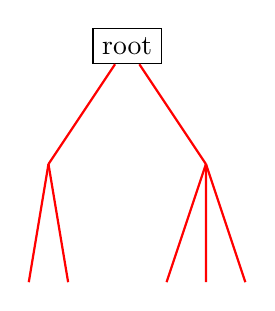
\begin{tikzpicture}
  \tikzstyle{level 1}=[sibling distance=20mm]
  \tikzstyle{level 2}=[sibling distance=5mm]
  \node {root}
    child { child child }
    child { child child child };
\end{tikzpicture}
\end{codeexample}
\end{itemize}




\subsection{Placing Child Nodes}

\label{section-tree-placement}

Perhaps the most difficult part in drawing a tree is the correct
layout of the children. Typically, the children have different sizes
and it is not easy to arrange them in such a manner that not too much
space is wasted, the children do not overlap, and they are either 
evenly spaced or their centers are evenly distributed. Calculating
good positions is especially difficult since a good position for the
first child may depend on the size of the last child.

In \tikzname, a comparatively simple approach is taken to placing the
children. In order to compute a child's position, all that is taken
into account is the number of the current child in the list of
children and the number of children in this list. Thus, if a node has
five children, then there is a fixed position for the first child, a
position for the second child, and so on. These positions \emph{do not
  depend on the size of the children} and, hence, children can easily
overlap. However, since you can use options to shift individual
children a bit, this is not as great a problem as it may seem.

Although the placement of the children only depends on their number in
the list of children and the total number of children, everything else
about the placement is highly configurable. You can change the
distance between children (appropriately called the
|sibling distance|) and the distance between levels of the tree. These
distances may change from level to level. The direction in which the
tree grows can be changed globally and for parts of the tree. You can
even specify your own ``growth function'' to arrange children on a
circle or along special lines or curves. 

The default growth function works as follows: Assume that we are given
a node and five children. These children will be placed on a line with
their centers (or, more generally, with their anchors) spaced apart by
the current |sibling distance|. The line is 
orthogonal to the current \emph{direction of growth}, which is set
with the |grow| and |grow'| option (the latter option reverses the
ordering of the children). The distance from the line to the parent node
is given by the |level distance|.

{\catcode`\|=12
\begin{codeexample}[]
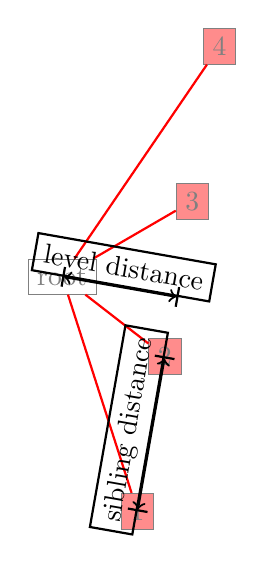
\begin{tikzpicture}
  \path [help lines]
    node (root) {root}
    [grow=-10]
    child {node {1}}
    child {node {2}}
    child {node {3}}
    child {node {4}};

  \draw[|<->|,thick] (root-1.center)
    -- node[above,sloped] {sibling distance} (root-2.center);

  \draw[|<->|,thick] (root.center) 
    -- node[above,sloped] {level distance} +(-10:\tikzleveldistance);
\end{tikzpicture}
\end{codeexample}
}

Here is a detailed description of the options:
\begin{itemize}
  \itemoption{level distance}|=|\meta{distance}
  This option allows you to change the distance between different
  levels of the tree, more precisely, between the parent and the line
  on which its children are arranged. When given to a single child,
  this will set the distance for this child only.
 
\begin{codeexample}[]
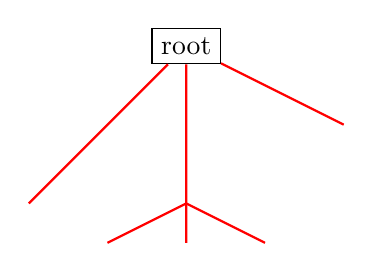
\begin{tikzpicture}
  \node {root}
    [level distance=20mm]
    child
    child {
      [level distance=5mm]
      child
      child
      child
    }
    child[level distance=10mm];  
\end{tikzpicture}
\end{codeexample}
 
\begin{codeexample}[]
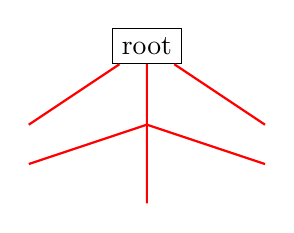
\begin{tikzpicture}
  \tikzstyle{level 1}=[level distance=10mm]    
  \tikzstyle{level 2}=[level distance=5mm]    
  \node {root}
    child
    child {
      child
      child[level distance=10mm]
      child
    }
    child;
\end{tikzpicture}
\end{codeexample}

  \itemoption{sibling distance}|=|\meta{distance}
  This option specifies the distance between the anchors of the
  children of a parent node.   

\begin{codeexample}[]
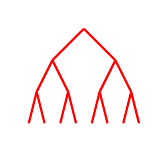
\begin{tikzpicture}[level distance=4mm]
  \tikzstyle{level 1}=[sibling distance=8mm]
  \tikzstyle{level 2}=[sibling distance=4mm]
  \tikzstyle{level 3}=[sibling distance=2mm]
  \coordinate
     child {
       child {child child}
       child {child child}
     }
     child {
       child {child child}
       child {child child}
     };
\end{tikzpicture}
\end{codeexample}

\begin{codeexample}[]
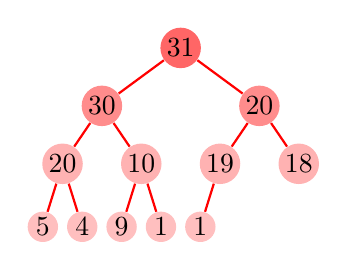
\begin{tikzpicture}[level distance=10mm]
  \tikzstyle{every node}=[fill=red!60,circle,inner sep=1pt]
  \tikzstyle{level 1}=[sibling distance=20mm,nodes={fill=red!45}]
  \tikzstyle{level 2}=[sibling distance=10mm,nodes={fill=red!30}]
  \tikzstyle{level 3}=[sibling distance=5mm,nodes={fill=red!25}]
  \node {31}
     child {node {30}
       child {node {20}
         child {node {5}}
         child {node {4}}
       }
       child {node {10}
         child {node {9}}
         child {node {1}}
       }
     }
     child {node {20}
       child {node {19}
         child {node {1}}
         child[fill=none] {edge from parent[draw=none]}
       }
       child {node {18}}
     };
\end{tikzpicture}
\end{codeexample}
  
  \itemoption{grow}|=|\meta{direction}
  This option is used to define the \meta{direction} in which the tree
  will grow. The \meta{direction} can either be an angle in degrees or
  one of the following special text strings: |down|, |up|, |left|,
  |right|, |north|, |south|, |east|, |west|, |north east|,
  |north west|, |south east|, and |south west|. All of these have
  ``their obvious meaning,'' so, say, |south west| is the same as the
  angle $-135^\circ$.

  As a side effect, this option installs the default growth function.

  In addition to setting the direction, this option also has a
  seemingly strange effect: It sets the sibling distance for the
  current level to |0pt|, but leaves the sibling distance for later
  levels unchanged.

  This somewhat strange behaviour has a highly desirable effect: If
  you give this option before the list of children of a node starts,
  the ``current level'' is still the parent level. Each child will be
  on a later level and, hence, the sibling distance will be as
  specified originally. This will cause the children to be neatly
  aligned in a line orthogonal to the given \meta{direction}. However,
  if you give this option locally to a single child, then ``current
  level'' will be the same as the child's level. The zero sibling
  distance will then cause the child to be placed exactly at a point
  at distance |level distance| in the direction
  \meta{direction}. However, the children of the child will be placed
  ``normally'' on a line orthogonal to the \meta{direction}.

  These placement effects are best demonstrated by some examples:
\begin{codeexample}[]
\tikz \node {root} [grow=right] child child;
\end{codeexample}

\begin{codeexample}[]
\tikz \node {root} [grow=south west] child child;
\end{codeexample}

\begin{codeexample}[]
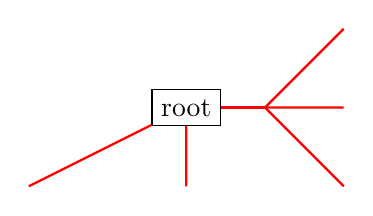
\begin{tikzpicture}[level distance=10mm,sibling distance=5mm]
  \node {root}
    [grow=down]
    child
    child
    child[grow=right] {
      child child child
    };  
\end{tikzpicture}
\end{codeexample}

\begin{codeexample}[]
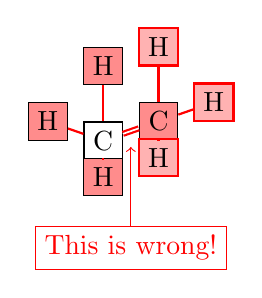
\begin{tikzpicture}[level distance=2em]
  \node {C}
    child[grow=up]    {node {H}}
    child[grow=left]  {node {H}}
    child[grow=down]  {node {H}}
    child[grow=right] {node {C}
        child[grow=up]    {node {H}}
        child[grow=right] {node {H}}
        child[grow=down]  {node {H}}
      edge from parent[double]
        coordinate (wrong)
    };
  \draw[<-,red] ([yshift=-2mm]wrong) -- +(0,-1)
    node[below]{This is wrong!};  
\end{tikzpicture}
\end{codeexample}

\begin{codeexample}[]
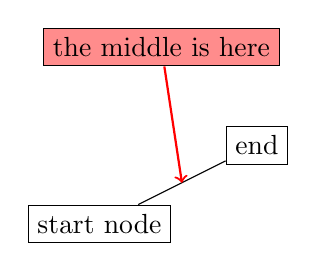
\begin{tikzpicture}
  \node[rectangle,draw] (a) at (0,0) {start node};
  \node[rectangle,draw] (b) at (2,1) {end};

  \draw (a) -- (b)
    node[coordinate,midway] {}
      child[grow=100,<-] {node[above] {the middle is here}};
\end{tikzpicture}
\end{codeexample}

  \itemoption{grow'}|=|\meta{direction}
  This option has the same effect as |grow|, only the children are
  arranged in the opposite order.

  \itemoption{growth parent anchor}|=|\meta{anchor}
  This option allows you to specify which anchor of the parent node is
  to be used for computing the children's position. For example, when
  there is only one child and the |level distance| is |2cm|, then the
  child node will be placed two centimeters below the \meta{anchor} of
  the parent node. ``Beinng placed'' means that the child node's
  anchor (which is the anchor specified using the |anchor=| option in
  the |node| command of the child) is two centimeters below the parent
  node's \meta{anchor}. The default value of \meta{anchor} is
  |center|.

  In the following example, the two red lines both have length |1cm|.
\begin{codeexample}[]
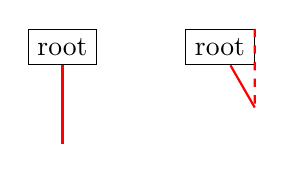
\begin{tikzpicture}[level distance=1cm]
  \node [rectangle,draw] (a) at (0,0) {root}
  [growth parent anchor=south] child;

  \node [rectangle,draw] (b) at (2,0) {root}
  [growth parent anchor=north east] child;

  \draw [red,thick,dashed] (a.south) -- (a-1);
  \draw [red,thick,dashed] (b.north east) -- (b-1);
\end{tikzpicture}
\end{codeexample}

  In the next example, the top and bottom nodes are aligned at the top
  and the bottom.
\begin{codeexample}[]
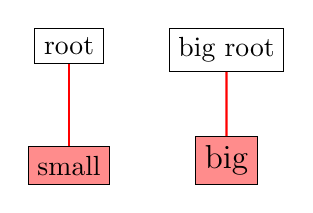
\begin{tikzpicture}[level distance=2cm,growth parent anchor=north]
  \tikzstyle{every node}=[anchor=north,rectangle,draw]    
  \tikzstyle{every child node}=[anchor=south]

  \node at (0,0) {root} child {node {small}};

  \node at (2,0) {big root} child {node {\large big}};
\end{tikzpicture}
\end{codeexample}

  \itemoption{growth function}|=|\meta{macro name}
  This rather low-level option allows you to set a new growth
  function. The \meta{macro name} must be the name of a macro without
  parameters. This macro will be called for each child of a node.

  The effect of executing the macro should be the following: It should
  transform the coordinate system in such a way that the origin
  becomes the place where the current child should be anchored. When
  the macro is called, the current coordinate system will be setup
  such that the anchor of the parent node is in the origin. Thus, in
  each call, the \meta{macro name} must essentially do a shift to the
  child's origin. When the macro is called, the \TeX\ counter
  |\tikznumberofchildren| will be set to the total number of children
  of the parent node and the counter |\tikznumberofcurrentchild| will
  be set to the number of the current child.

  The macro may, in addition to shifting the coordinate system, also
  transform the coordinate system further. For example, it could be
  rotated or scaled.

  Additional growth functions are defined in the library, see 
  Section~\ref{section-tree-library}.
\end{itemize}



\subsection{Edges From the Parent Node}

\label{section-edge-from-parent}

Every child node is connected to its parent node via a special kind of
edge called the |edge from parent|. This edge is added to the
\meta{child path} when the following path operation is encountered:

\begin{pathoperation}{edge from parent}{\opt{\oarg{options}}}
  This path operation can only be used inside \meta{child paths} and
  should be given at the end, possibly followed by node specifications
  (we will come to that). If a \meta{child path} does not contain this
  operation, it will be added at the end of the \meta{child path}
  automatically.

  This operation has several effects. The most important is that it
  inserts the current ``edge from parent path'' into the child
  path. The edge from parent path can be set using the following
  option:
  \begin{itemize}
    \itemoption{edge from parent path}|=|\meta{path}
    This options allows you to set the edge from parent path to a new
    path. The default for this path is the following:
    \begin{codeexample}[code only]
(\tikzparentnode\tikzparentanchor) -- (\tikzchildnode\tikzchildanchor)      
    \end{codeexample}
    The |\tikzparentnode| is a macro that will expand to the name of
    the parent node. This works even when you have not assigned a name
    to the parent node, in this case an internal name is automatically
    generated. The |\tikzchildnode| is a macro that expands to the
    name of the child node. The two |...anchor| macros are empty by
    default. So, what is essentially inserted is just the path segment
    |(\tikzparentnode) -- (\tikzchildnode)|; which is exactly an edge
    from the parent to the child.

    You can modify this edge from parent path to achieve all sorts of
    effects. For example, we could replace the straight line by a
    curve as follows:
\begin{codeexample}[]
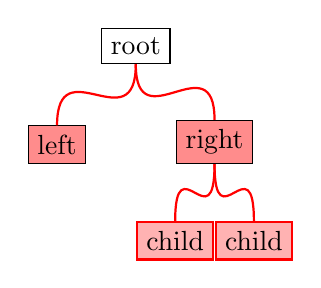
\begin{tikzpicture}[edge from parent path=
  {(\tikzparentnode.south) .. controls +(0,-1) and +(0,1)
                           .. (\tikzchildnode.north)}]
  \node {root}
    child {node {left}}
    child {node {right}
      child {node {child}}
      child {node {child}}
    };
\end{tikzpicture}
\end{codeexample}

    Further useful edge from parent paths are defined in the tree
    library, see Section~\ref{section-tree-library}.

    As said before, the anchors in the default edge from parent path
    are empty. However, you can set them using the following options:
    \begin{itemize}
      \itemoption{child anchor}|=|\meta{anchor}
      Specifies the anchor where the edge from parent meets the child
      node by setting the macro |\tikzchildanchor| to
      |.|\meta{anchor}.

      If you specify |border| as the \meta{anchor}, then the macro
      |\tikzchildanchor| is set to the empty string. The effect of
      this is that the edge from the parent will meet the child on the
      border at an automatically calculated position.
\begin{codeexample}[]
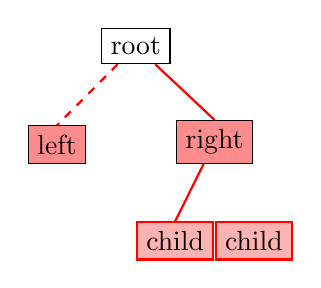
\begin{tikzpicture}
  \node {root}
    [child anchor=north]
    child {node {left} edge from parent[dashed]}
    child {node {right}
      child {node {child}}
      child {node {child} edge from parent[draw=none]}
    };
\end{tikzpicture}
\end{codeexample}
      \itemoption{parent anchor}|=|\meta{anchor}
      This option works the same way as the |child anchor|, only for
      the parent.
    \end{itemize}
  \end{itemize}

  Besides inserting the edge from parent path, the |edge from parent|
  operation has another effect: The \meta{options} are inserted
  directly before the edge from parent path and the following style is
  also installed prior to inserting the path:
  \begin{itemize}
    \itemstyle{edge from parent}
    This style is inserted right before the edge from parent path and
    before the \meta{options} are inserted. By default, it just draws
    the edge from parent, but you can use it to make the edge look
    different. 
\begin{codeexample}[]
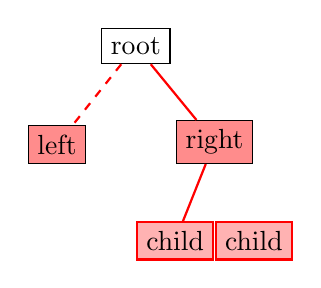
\begin{tikzpicture}
  \tikzstyle{edge from parent}=[draw,red,thick]    
  \node {root}
    child {node {left} edge from parent[dashed]}
    child {node {right}
      child {node {child}}
      child {node {child} edge from parent[draw=none]}
    };
\end{tikzpicture}
\end{codeexample}
  \end{itemize}

  Note: The \meta{options} inserted before the edge from parent path
  is added \emph{apply to the whole child path}. Thus, it is not
  possible to, say, draw a circle in red as part of the child path and
  then have an edge to parent in blue. However, as always, the child
  node is a node and can be drawn in a totally different way.

  Finally, the |edge from parent| operation has one more effect: It
  causes all nodes \emph{following} the operation to be placed on the
  edge. This is the same effect as if you had added the |pos| option
  to all these nodes, see also Section~\ref{section-pos-option}.

  As an example, consider the following code:
\begin{codeexample}[code only]
\node (root) {} child {node (child) {} edge to parent node {label}};    
\end{codeexample}
  The |edge to parent| operation and the following |node| operation
  will, together, have the same effect as if we had said:
\begin{codeexample}[code only]
(root) -- (child) node [pos=0.5] {label}
\end{codeexample}

  Here is a more complicated example:
\begin{codeexample}[]
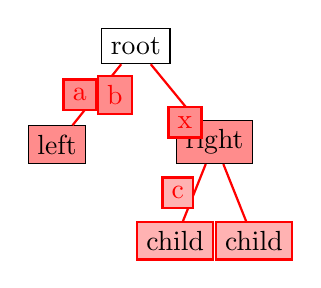
\begin{tikzpicture}
  \node {root}
    child {
      node {left}
      edge from parent
        node[left] {a}
        node[right] {b}
    }
    child {
      node {right}
        child {
          node {child}
          edge from parent
            node[left] {c}
        }
        child {node {child}}
      edge from parent
        node[near end] {x}
    };
\end{tikzpicture}
\end{codeexample}

\end{pathoperation}



%%% Local Variables: 
%%% mode: latex
%%% TeX-master: "pgfmanual-pdftex-version"
%%% End: 
